\section{Model and Exact Formula}
In this section, we explain the model which describes the heat transport via a local two-state system.
Then, we derive the exact formula of liner heat conductance in this system by using the Keldysh formalism.

When we discuss the heat transport via a zero-dimensional object, we should consider the system where a local oscillator is localized between two phonon baths. 
Now, we adopt the double well potential as the local oscillator because this potential can denote the boson interaction caused by nonlinearity. In reality, this system can be implemented as the molecular junction or the Josephson junction in the super conducting circuit\cite{experiment?}(Fig. \ref{fig:j_c}).
\begin{figure}[tb]
	\centering
	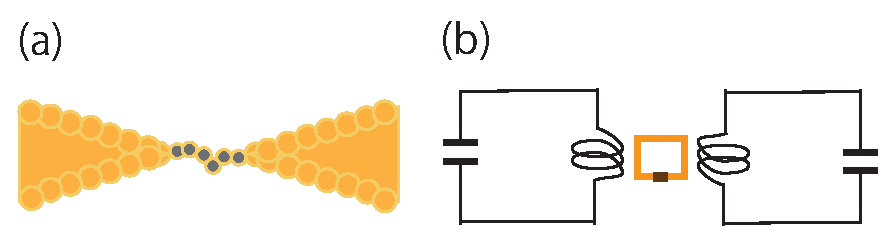
\includegraphics[width=130mm]{j_c.eps}
	\caption{(a)molecular junction, (b)Josephson junction in the super conducting circuit}
	\label{fig:j_c}
\end{figure}
At low temperature, when the potential barrier is infinitely higher than the energy level difference from the ground state to the first excited state, the local oscillator can be regarded as the two-state system described by the ground state where the system is localized at the right or left well.
Then, we can relate the two-state system to the pseudo-spin system. 
Then, the Hamiltonian of local oscillator is described by  the Pauli matrix $\sigma_{i}(i:x,y,z)$ as
\begin{eqnarray}
	H=\frac{\hbar \Delta}{2} \sigma_x+\frac{\hbar\epsilon}{2}\sigma_z,
\end{eqnarray}
where $\Delta$ is the tunneling amplitude and $\epsilon$ is the bias of the system, i.e., the difference in the ground-state energies of the local two states.
In this study, we assume the symmetric double well, i.e., $\epsilon=0$.
Then, the local two-state system coupling to two phononic baths is described by the spin-boson Hamiltonian:
\begin{eqnarray}
	H=\frac{\hbar \Delta}{2} \sigma_x 
	+\sum_{\nu=L,R}\sum_{\nu k}\hbar \omega_{\nu k } b_{\nu k}^{\dagger} b_{\nu k}
	+ \frac{\sigma_z}{2} \sum_{\nu=L,R}\sum_{\nu k} \hbar \lambda_{\nu k}(b_{\nu k}+b_{\nu k}^{\dagger}),
	\label{Hamiltonian}
\end{eqnarray}
where $\omega_{\nu k}$, $b_{\nu k}$ is the frequency and annihilation operator of phonon with the wavenumber $k$ in the $\nu$th bath, and $\lambda_{\nu k}$ is the coupling strength between the local two-state system and phonons in two phononic baths.
(Fig. \ref{fig:system_image}) is the image? of this system.
\begin{figure}[tb]
	\centering
	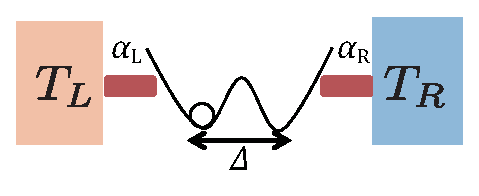
\includegraphics[width=100mm]{system_image.eps}
	\caption{The two-state system coupling to two phononic baths. If the temperature of two baths is slightly different, phonon can be transported from one bath to another.}
	\label{fig:system_image}
\end{figure}
The spectral function defined as  
\begin{eqnarray}
	I_{\nu}(\omega)&\equiv&\sum_{\nu k} \lambda_{\nu k}^2\delta(\omega-\omega_{\nu k})
\end{eqnarray}
characterizes the behavior of heat transport under the spin-boson model.
We assume that the spectral function takes the form of power law:
\begin{eqnarray}
	I_{\nu}(\omega)&=&\alpha_\nu \tilde{I}_\nu (\omega), \label{spect} \\
	\tilde{I}_\nu(\omega)&=&2\omega_c^{1-s}\omega^s f(\omega/\omega_c),
\end{eqnarray}
where $\alpha_{\nu}$ is the dimensionless coupling strength between the local two-state system and the $\nu$th heat bath, $\omega_c$ is the cutoff frequency satisfying $\omega_c\gg\Delta,\epsilon$, and $f(\omega/\omega_c)$ is the cutoff function in the range [0,1]. For simplicity, we assume the cutoff function $f(\omega/\omega_c)$ takes the form of step function $\theta(\omega_c-\omega)$.
The case of $s=1$ is called ``ohmic'' and the ohmic case is studied in detail as we discussed in the section 1. 
The case of $s>1$ and $ s<1$ is called ``super-ohmic" and ``sub-ohmic", respectively, 
and these non-ohmic case is our main interest.
Starting with this setup, we derive the exact formula of thermal conductance under the spin-boson model by using Keldysh formalism.
 
First, we define the operator of the heat current flowing from the $\nu$th bath into the local two-state system as 
\begin{eqnarray}
	J_\nu\equiv\frac{dH_{\mathrm{bath},\nu}}{dt},
	\label{current_opperator}
\end{eqnarray}
where the Hamiltonian of the $\nu$th bath is defined as $H_{\mathrm{bath},\nu} \equiv\sum_k\hbar \omega_{\nu k } b_{\nu k}^{\dagger} b_{\nu k}$.
This operator follows the Heisenberg's equation of motion, then 
\begin{eqnarray}
	J_\nu&=&-\frac{i}{\hbar}[H_{\mathrm{bath},\nu},H]\\
	&=&-i \sum_k\frac{\lambda_{\nu k}}{2}\hbar\omega_{\nu k}\sigma_z(-b_{\nu k}+b_{\nu k}^{\dagger}).
\end{eqnarray}
The ensemble average of heat current $\average{J_\nu(t)}=\mathrm{Tr}[\rho J_\nu(t)]$, where $\rho$ is the density matrix of initial state, is calculated as 
\begin{eqnarray}
	\average{J_\nu(t)}=\mathrm{Re}\left . \left[\sum_k\frac{\hbar^2\omega_{\nu k} \lambda_{\nu k}}{2}
	G^{<}_{\sigma_z,b_{\nu k}^{\dagger}}(t_1,t_2)\right] \right |_{t_1=t_2=t},
\end{eqnarray}
where the lesser Green's function is defined as 
\begin{eqnarray}
	G^{<}_{\sigma_z,b_{\nu k}^{\dagger}}(t_1,t_2)\equiv-\frac{i}{\hbar}\average{b_{\nu k}^{\dagger}(t_2)\sigma_z(t_1)}.
\end{eqnarray}
Then, by using Keldysh formalism, we can derive the heat current at the steady state\cite{Saito08}:
\begin{eqnarray}
	\average{J_\nu}=\frac{\hbar}{4}\int_{0}^{\infty}d\omega\, 
		\hbar \omega\left[ 
			\mathrm{Im}[G_{\sigma_z,\sigma_z}^{r}(\omega)]I_\nu(\omega)n_\nu( \hbar\omega)-
			iG^{<}_{\sigma_z,\sigma_z}(\omega)\frac{I_\nu(\omega)}{2}
		\right],
\end{eqnarray}
where  $n_\nu( \hbar\omega)$ means the Bose-Einstein distribution function and the retarded Green's function is defined as 
\begin{eqnarray}
	G_{A,B}^r(t_1,t_2)\equiv -\frac{i}{\hbar}\theta(t_1-t_2)\average{[A(t_1),B(t_2)]}.
\end{eqnarray}
Here, we introduce the quantity $\gamma_\nu$ which denotes the symmetry of coupling to the two baths:
\begin{eqnarray}
	\gamma_\nu=\frac{\int_0^{\infty}d\omega\,\hbar\omega G_{\sigma_z,\sigma_z}^{<}(\omega)I_\nu(\omega)}	{\sum_{\nu'=L,R}\int_{0}^{\infty}d\omega\,\hbar\omega G_{\sigma_z,\sigma_z}^<(\omega)I_{\nu'}(\omega)}.
\end{eqnarray}
Remarking the conservation law of the particle number $\average{J _L}+\average{J_R}=0$, $\average{J_L}$ can be denoted as follows by $\gamma_{\nu}$
\begin{eqnarray}
	\average{J _L}&=&\gamma_R\average{J_L}-\gamma_L\average{J_R}\\
	&=&\frac{1}{4}\int_0^{\infty}d(\hbar\omega)\,
	\hbar\omega\mathrm{Im}[G^r_{\sigma_z,\sigma_z}(\omega)]
	\left[\gamma_RI_L(\omega)n_L(\hbar\omega)-\gamma_LI_R(\omega)n_R(\hbar\omega)\right].
\end{eqnarray}
Here, we assume $\tilde{I}_L(\omega)=\tilde{I}_R(\omega)=\tilde{I}(\omega)$, then $\average{J_L}$ is
\begin{eqnarray}
	\average{J _L}=\frac{\alpha_L\alpha_R}{4(\alpha_L+\alpha_R)}\int_0^{\infty}d(\hbar\omega)
		\hbar\omega\mathrm{Im}[G^r_{\sigma_z,\sigma_z}(\omega)]
		\tilde{I }(\omega)\left[n_L(\hbar\omega)-n_R(\hbar\omega)\right].
		\label{exact_current}
\end{eqnarray}
In the linear response regime, thermal conductance is defined as
\begin{eqnarray}
	\kappa\equiv \lim_{\Delta T \rightarrow 0} \frac{\average{J_L}}{\Delta T}.
	\label{den_kappa}
\end{eqnarray}
Finally, we can get the exact formula of thermal conductance: 
\begin{eqnarray}
	\kappa=\frac{k_B\alpha\omega_c^{1-s}}{4}\int_{0}^{\infty}d(\hbar\omega)\mathrm{Im}
	[\chi(\omega)]\omega^s\left[\frac{\beta\hbar\omega/2}{\mathrm{sinh}(\beta\hbar\omega/2)}\right]^2,
	\label{exact_kappa}
\end{eqnarray}
where we assumed  the symmetric coupling strength $\alpha=\alpha_L=\alpha_R$ and substituted the response function $\chi(\omega)$ for $G^r_{\sigma_z,\sigma_z}(\omega)$ by considering the linear response theory.
Eq. (\ref{exact_kappa}) is the main result in this section.
When we evaluate the value of conductance (\ref{exact_kappa}), we have to calculate the response function $\mathrm{Im}[{\chi}(\omega)]$. But, except the special case like ``Toulouse limit'' ($\alpha=1/2$ in the ohmic case), it is difficult to analytically calculate $\mathrm{Im}[{\chi}(\omega)]$.
Here, in this study, we numerically evaluate $\mathrm{Im}[{\chi}(\omega)]$ by the Monte Carlo method.
Although we explain how to numerically calculate $\mathrm{Im}[{\chi}(\omega)]$ in section 4 in detail,
in the next section, we derive the approximate formulas of thermal conductance (\ref{exact_kappa}) in three different situations.  